% !TEX root = ./notes.tex
\chapter[Stellar Atmospheres]{Stellar Atmospheres}
\label{s.stellar-atmospheres}

In the atmosphere of the star, the optical depth approaches unity, and we can no longer treat the radiation field as being isotropic. Let's consider the time-independent problem ($\partial_{t}\to 0$) of a plane-parallel atmosphere. The \emph{optical depth} for an outward-directed ray is
\begin{equation}\label{e.optical-depth}
\tau_{\nu} = \int _{z}^{\infty}\!\rho\kappa_{\nu}\,\dif z'.
\end{equation}
Now the optical depth just the distance divided by the mean free path. Clearly, when $\tau_{\nu} < 1$, a photon has a good chance of reaching a distant observer without any further interactions with the stellar matter.  As a result, the intensity takes its final form around $\tau_{\nu} \approx 1$, and this defines the stellar \emph{photosphere}. To get some of the basic properties of the photosphere, rewrite eq.~(\ref{e.optical-depth}) in differential form,
\begin{equation}\label{e.dtaudz}
\frac{\dif\tau}{\dif z} = -\rho\kappa.
\end{equation}
This is for a crude estimate, so we neglect the frequency dependence for now.  We can use equation~(\ref{e.dtaudz}) along with hydrostatic balance to get an estimate of the photospheric pressure,
\begin{equation}\label{e.photo-pressure}
\frac{\dif P}{\dif \tau} = -\left(\frac{\dif \tau}{\dif z}\right)^{-1}\rho g = \frac{g}{\kappa}.
\end{equation}
Thus, at $\tau \approx 1$, the pressure is $P_{\mathrm{ph}}\approx g/\kappa$. Since the flux at the photosphere is $\ssb \Teff^{4}$, we would expect that the local temperature is $T\approx \Teff$.

\section{The Eddington Approximation}

To get an analytical approximation for the atmosphere, we'll first redefine our transfer equation in terms of optical depth (eq.~[\ref{e.transfer-with-source}]). Here however, we will take the optical depth to be along the $z$-direction, so we define $\mu = \unitk\vdot\unitn$, where \unitn\ is the direction along the ray. The equation of transfer then becomes
\begin{equation}\label{e.planar}
\mu\frac{\partial I_{\nu}}{\partial\tau_{\nu}} = I_{\nu}-S_{\nu},
\end{equation}
where 
\begin{equation}\label{e.source}
S_{\nu} \equiv \frac{1}{\kappa_{\nu}}\left(\frac{\varepsilon_{\nu}}{4\pi} + \kappa_{\nu}^{\mathrm{sca}}J_{\nu}\right)
\end{equation}
is the \emph{source function}. In local thermodynamical equilibrium (LTE), we can write $S_{\nu} = (1-A_{\nu})B_{\nu} + A_{\nu}J_{\nu}$, where $A_{\nu} \equiv \kappa_{\nu}^{\mathrm{sca}}/\kappa_{\nu}$ is the \emph{albedo}.  Recall that $J_{\nu} = (4\pi)^{-1}\int\dif\Omega\,I_{\nu}$ is the angle-average of $I_{\nu}$.

We noted that in thermal equilibrium, $P_{\nu} = c^{-1}\int_{-1}^{1}\dif\mu\,\mu^{2}I_{\nu} = u_{\nu}/3$. This relation holds even when the radiation is not thermal, so long as it is isotropic to terms linear in $\mu$.  To make this concrete, suppose we write
\[ I_{\nu}(\mu) = I_{\nu}^{(0)} + \mu I_{\nu}^{(1)} + \mu^{2}I_{\nu}^{(2)} + \ldots. \]
Here we are assuming that terms marked $(0)$ are much larger than terms marked $(1)$, etc.  To lowest order, the energy density, flux, and momentum flux are then
\begin{eqnarray*}
u_{\nu} &=& \frac{2\pi}{c}\int_{-1}^{1}\dif\mu\,I_{\nu}(\mu) = \frac{4\pi}{c} I_{\nu}^{(0)},\\
F_{\nu} &=& 2\pi\int_{-1}^{1}\dif\mu\,\mu\,I_{\nu}(\mu) = \frac{4\pi}{3} I_{\nu}^{(1)},\\
P_{\nu} &=& \frac{2\pi}{c}\int_{-1}^{1}\dif\mu\,\mu^{2}\,I_{\nu}(\mu) = \frac{4\pi}{3c}I_{\nu}^{(0)} = \frac{u_{\nu}}{3}.
\end{eqnarray*}
The \emph{Eddington approximation} then consists of treating the radiation field as if its anisotropy is linear in $\mu$ \emph{everywhere}, so that the above relations hold; in particular, it means assuming that $P_{\nu} = u_{\nu}/3$ everywhere.

\section[Grey Atmosphere]{A Grey Atmosphere}

Finally, to get an analytical approximation to the structure of the solar atmosphere, let's consider a grey atmosphere in LTE, i. e., one for which $\kappa_{\nu}^{\mathrm{abs}} = \kappa^{\mathrm{abs}}$ and $\kappa_{\nu}^{\mathrm{sca}} = \kappa^{\mathrm{sca}}$ are independent of frequency. Equation~(\ref{e.planar}) can then be integrated over all frequencies to become
\begin{equation}\label{e.J-grey}
\mu\frac{\partial I}{\partial\tau} = I-S.
\end{equation}
Integrating over all angles (note that we can pull the derivative wrt $\tau$ out of the integral) gives
\begin{equation}\label{e.H-grey}
\frac{1}{4\pi}\frac{\partial F}{\partial\tau} = J - S = 0.
\end{equation}
Why does the right-hand side vanish? Note that $S-J = (1-A)(B-J)$.  Clearly $S = J$ if $A = 1$ (a pure scattering atmosphere).  If $A \ne 1$, so that there is some absorption, then the condition of detailed balance, equation~(\ref{e.detail-balance}), implies that $\varepsilon_{\nu} = 4\pi\kappa^{\mathrm{abs}}B_{\nu}(T)$; inserting this into equation~(\ref{e.rad-equil}), factoring out the constant $\kappa^{\mathrm{abs}}$, and integrating over $\nu$ implies that $B - J = 0$, and hence $S - J = 0$. Note that $J = B$ does \emph{not} necessarily imply that $I_{\nu} = B_{\nu}$!

Now multiply equation~(\ref{e.J-grey}) by $\mu$ and integrate over $2\pi\,\dif\mu$ to obtain
\begin{equation}\label{e.K-grey}
c\frac{\partial P}{\partial\tau} = F,
\end{equation}
the integral over $\mu S$ vanishing because it is odd in $\mu$. Equation~(\ref{e.H-grey}) implies that $F$ is constant; hence we can integrate equation~(\ref{e.K-grey}) at once to obtain
\begin{equation}\label{e.KH}
cP = F(\tau + \tau_{0}),
\end{equation}
where $\tau_{0}$ is a constant of integration. Of course, this does help us yet; all we have done is introduce a new variable $P$, the radiation pressure. This is where the Eddington approximation comes in.  We set $P = u/3 = 4\pi J/(3c)$ in equation~(\ref{e.KH}) to obtain $4\pi J = 3F(\tau + \tau_{0})$. Since $J = S$, we can then write equation~(\ref{e.J-grey}) as
\begin{equation}
\mu\frac{\partial I}{\partial\tau} = I - \frac{3}{4\pi}F(\tau+\tau_{0}).
\end{equation}
Since $F$ is constant, this first-order differential equation is now solvable,
\begin{eqnarray}
I(\mu,\tau=0) &=& \frac{1}{\mu}\int_{0}^{\infty}\!\frac{3}{4\pi}F(\tau + \tau_{0}) e^{-\tau/\mu}\,\dif\tau,\nonumber\\
  &=& \frac{3}{4\pi}F(\mu + \tau_{0}).\label{e.I-Edd}
\end{eqnarray}
Now at $\tau = 0$, all of the flux must be outward-directed ($\mu >0$), so $I(\mu < 0,\tau = 0) = 0$ if the star is not irradiated by another source.  Note that the Eddington approximation is clearly violated here.  Still, we will see later that this approximation is not too terrible. 

To determine $\tau_{0}$, multiply $I(\mu,\tau = 0)$ by $\mu$ and integrate equation~(\ref{e.I-Edd}) over all angles to find
\begin{equation}
F = 2\pi\int_{0}^{1}\!\mu I(\mu,0)\,\dif\mu = \frac{1}{2}\int_{0}^{1}\!3F(\mu + \tau_{0})\,\mu\,\dif\mu = F\left(\frac{1}{2} + \frac{3}{4}\tau_{0}\right).
\end{equation}
We therefore find $\tau_{0} = 2/3$. Now, since we are in LTE, $P = aT^{4}/3$. Further, let us define an effective temperature by the relation $F = \ssb\Teff^{4}$.  Substituting these definitions and the value of $\tau_{0}$ into equation~(\ref{e.KH}) gives us the atmospheric temperature structure,
\begin{equation}\label{e.Eddington}
T^{4}(\tau) = \frac{3}{4}\Teff^{4}\left(\tau + \frac{2}{3}\right).
\end{equation}
Thus $T(\tau  = 0) = 2^{-1/4} \Teff$ and $T(\tau = 2/3) = \Teff$.  

\begin{figure}[htbp]
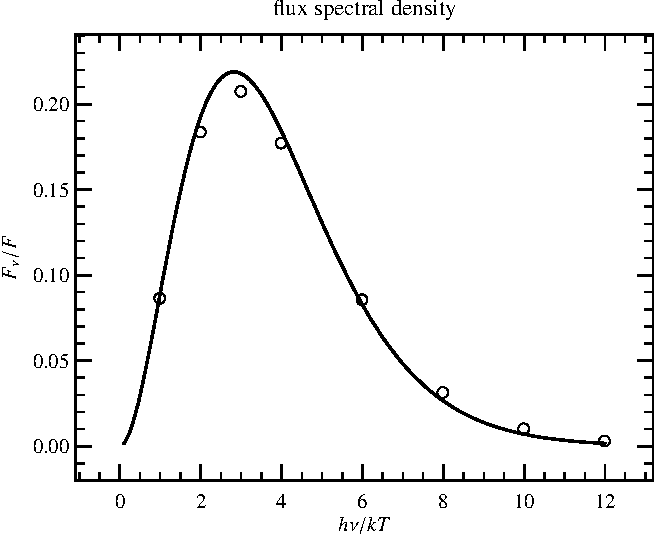
\includegraphics[width=4in]{Figures/plots_out/spectral_distribution}
\caption{\label{f.spectral} Spectral distribution from a grey atmosphere. The open circles are from Chandrasekhar, \emph{Radiative Transfer}; the solid line is the Planck distribution.}
\end{figure}

To get the spectral distribution, go back to equation~(\ref{e.planar}) and (assuming the atmosphere has some absorption so that the matter and radiation can come into equilibrium) insert $S_{\nu} = B_{\nu}(T)$; solving for $I_{\nu}$ at $\tau = 0$ then gives
\begin{equation}\label{e.spectral}
I_{\nu}(\mu,\tau=0) = \frac{1}{\mu}\int_{0}^{\infty}\!B_{\nu}\left[T(\tau)\right] \, e^{-\tau/\mu}\,\dif\tau.
\end{equation}
A plot of the spectral distribution for the emergent flux is shown (\emph{open circles}) in Fig.~\ref{f.spectral}. For comparison, a plot of the Planck distribution (\emph{solid line}) is also shown. Both fluxes are normalized to the total flux.  Note that $I_{\nu}(\mu,\tau=0)$ depends on angle; rays propagating at a slant will have a lower intensity.  As a result, when we observe the sun, the edge of the visible disk appears darker than the center, a phenomenon known as \emph{limb darkening}.

\section{Some examples}

\subsection{Requirement for convection in the atmosphere}\label{s.atmosphere-convection}

Let's construct a simple atmosphere model using our temperature structure, eq.~(\ref{e.Eddington}).  Although we assume a grey opacity, we will let if vary with temperature and density, $\kappa(\rho,T) = \kappa_{0}\rho^{r}T^{s}$.  For an ideal gas, we can rewrite this in terms of pressure and temperature, $\kappa(P,T) = \kappa_{0} (\mu\mb/k)^{r}P^{r} T^{s-r}$.  Substituting this into equation~(\ref{e.photo-pressure}), and using equation~(\ref{e.Eddington}), we obtain,
\[
  \frac{\dif P}{\dif \tau} = \frac{g}{\kappa_{0}}\left(\frac{k}{\mu\mb}\right)^{r} P^{-r} \left[\frac{3}{4}\Teff^{4}\left(\tau + \frac{2}{3}\right)\right]^{(r-s)/4}.
\]
This is easily integrated: we'll take $P(\tau = 0) = 0$ and obtain
\[
  P(\tau) = (\mathrm{const})\tau^{(r-s+4)/4/(1+r)}
\]
so that
\begin{equation}\label{e.dlnPdtau}
  \frac{\dif \ln P}{\dif \tau} = \frac{r-s+4}{4(1+r)\tau}.
\end{equation}
For the temperature,
\begin{equation}\label{e.dlnTdtau}
 \frac{\dif\ln T}{\dif\tau} = \frac{1}{4}\frac{\dif\ln T^{4}}{\dif \tau} = \frac{1}{4(\tau + 2/3)}.
\end{equation}
We now combine eqn.~(\ref{e.dlnPdtau}) and (\ref{e.dlnTdtau}) to obtain
\begin{equation}\label{e.dlnTdlnP-atmosphere}
\frac{\dif \ln T}{\dif\ln P} = \left(\frac{1+r}{r-s +4}\right)\left(\frac{\tau}{\tau + 2/3}\right).
\end{equation}
For convection to happen, $\dif\ln T/\dif\ln P > (\partial\ln T/\partial\ln P)_{s} = 1/(1+n)$, where $n = 3/2$ for an ideal gas.  That is,
\begin{equation}\label{e.convection-will-happen}
 n > \frac{r-s + 4}{1+r} - 1 = \frac{3-s}{1+r},
\end{equation}
is required for convection to happen somewhere.  Table~\ref{t.rhs} illustrates the behavior of $\dif\ln T/\dif\ln P$ for various opacity sources.  The fact that the H$^{-}$ opacity increases with temperature forces the temperature gradient to steepen with increasing pressure and ensures that low-mass stars have outer convective zones.

\begin{table}[htbp]
\caption{Right-hand side of eq.~(\ref{e.convection-will-happen}) for various opacities}
\label{t.rhs}
\begin{center}
\begin{tabular}{lrrr}
\hline
source & $r$ & $s$ & $\frac{3-s}{1+r}$\\
\hline\hline
Thomson & $0$ & $0$ & $3$\\
free-free & $14$ & $-7/2$ & $13/4$\\
H$^{-}$ & $1/2$ & $9$ & $-4$\\
\hline
\end{tabular}
\end{center}
\end{table}

\subsection{An irradiated atmosphere}\label{s.two-stream}

Many extra-solar planets are in rather tight orbits and as a result are strongly irradiated.  The following example is a simplified treatment of \citet{Hummer1982The-effect-of-r} and \citet{Hubeny2003A-Possible-Bifu}. At a distance $D$ from the star, the luminous flux is $\ssb T_{\star}^{4}(R_{\star}/D)^{2}$. The incident intensity is then $(\ssb/\pi)WT_{\star}^{4}$, where $W = (R_{\star}/D)^{2}$, since this will give the flux when integrated over all forward directions. 

An classic approximation in stellar atmospheres is to write the intensity as a sum of two streams,
\begin{equation}\label{e.two-stream}
I_{\nu}(\mu) = I_{\nu}^{+}\delta\left(\mu-\frac{1}{\sqrt{3}}\right) + I_{\nu}^{-}\delta\left(\mu + \frac{1}{\sqrt{3}}\right).
\end{equation}
The reason for the choice of $\mu$ becomes apparent when we compute the mean intensity, the flux, and the pressure:
\begin{eqnarray*}
J_{\nu} &=& \frac{1}{4\pi}\int\!\dif\phi\,\dif\mu\; I_{\nu} = \frac{1}{2}\left(I_{\nu}^{+} + I_{\nu}^{-}\right)\\
F_{\nu} &=& \int\!\dif\phi\,\dif\mu\;\mu I_{\nu} = \frac{2\pi}{\sqrt{3}} \left( I_{\nu}^{+} - I_{\nu}^{-}\right)\\
P_{\nu} &=& \frac{1}{c} \int\!\dif\phi\,\dif\mu\;\mu^{2} I_{\nu} = \frac{2\pi}{3c}\left(I_{\nu}^{+} + I_{\nu}^{-}\right).\\
\end{eqnarray*}
You will recognize by comparing $P_{\nu}$ with $J_{\nu}$ that this formalism automatically satisfies the Eddington approximation, since $J_{\nu} = (c/4\pi)u_{\nu}$ (cf.\ \S~\ref{s.radiation-description} and eq.~[\ref{e.thermal}]).

Following the standard method, we take successive moments of our equation of transfer (for a grey atmosphere),
\[ \mu\frac{\dif I}{\dif \tau} = I-S, \]
to obtain
\begin{eqnarray}
\frac{\dif F}{\dif \tau} &=& 4\pi (J - S) \label{e.2streamF}\\
c\frac{\dif P}{\dif\tau} &=& F. \label{e.2streamP}
\end{eqnarray}
In LTE, $J - S = 0$ and therefore $F = \textrm{const}$.  We therefore integrate eq.~(\ref{e.2streamP}) and use the Eddington approximation, $cP = (4\pi/3)J$, to obtain
\begin{equation}\label{e.2stream-1}
J(\tau) = \frac{3}{4\pi} F \tau + J_{0}.
\end{equation}
To determine $J_{0}$, we use our two stream approximation to write $J_{0} = (\sqrt{3}/4\pi)F + I^{-}$.  Since $F$ is constant, we set it to its value at great depth in the star.  Let us characterize $F$ by temperature $T_{\mathrm{int}}$ via $F \equiv \ssb T_{\mathrm{int}}^{4}$.  Finally, we set $I^{-}$ to the incident intensity, $I^{-} = (\ssb/\pi)WT_{\star}^{4}$ and note that in radiative equilibrium, $J = B = (\ssb/\pi) T^{4}(\tau)$. Collecting terms, we have the equation for the temperature structure,
\begin{equation}\label{e.T-irradiated}
T^{4}(\tau) = \frac{3}{4} T_{\mathrm{int}}^{4}\left(\tau + \frac{1}{\sqrt{3}}\right) + W T_{\star}^{4}.
\end{equation}
If $WT_{\star} \gg T_{\mathrm{int}}$, then the temperature is nearly isothermal to a depth $\tau_{h} \approx W(T_{\star}/T_{\mathrm{int}})^{4}$.
The assumption of a grey atmosphere is, however, quite poor: the incident photons are peaked in the optical, whereas the local temperatures are in the infrared. Even taking a mean opacity is not sufficient.

\section{Line formation and the curve of growth}\label{s.curve-of-growth}

Spectral lines are the diagnostics of a stellar atmosphere's temperature, pressure, and composition.  We'll briefly treat here how the ambient conditions set the line shape.

\subsection{The classical oscillator}\label{s.classical-oscillator}

Suppose we have a classical charged harmonic oscillator.  The instantaneous power emitted by the oscillator is
\begin{equation}\label{e.larmor-power}
	 P(t) = \frac{2}{3}\frac{e^{2}}{c^{3}} |\dot{\vu}|^{2},
\end{equation}
and when averaged over a cycle is
\begin{equation}\label{e.oscillator-power}
	 \left\langle P(t) \right\rangle = \frac{e^{2}}{3c^{3}}x_{0}^{2} \omega^{4},
\end{equation}
since $\dot{\vu} = -\omega^{2}\bvec{x}_{0}\cos \omega t$. Since the oscillator is radiating, it is losing energy and is damped. Let us write the damping as $\bvec{F}_{\mathrm{rad}}\vdot \vu$ and integrate over a cycle,
\[  -\int_{t_{1}}^{t_{2}}\!\dif t\;\frac{2}{3}\frac{e^{2}}{c^{3}}\dot{\vu}\vdot\dot{\vu} 
	= -\left.\frac{2}{3}\frac{e^{2}}{c^{3}}\dot{\vu}\vdot\vu\right|_{t_{1}}^{t_{2}} 
	+ \frac{2}{3}\frac{e^{2}}{c^{3}} \int_{t_{1}}^{t_{2}}\!\dif t\;\ddot{\vu}\vdot\vu. 
\]
The first term vanishes and we can therefore identify 
\[ 
	\bvec{F}_{\mathrm{rad}} = \frac{2}{3}\frac{e^{2}}{c^{3}}\ddot{\vu} 
	= -m\left(\frac{2e^{2}\omega^{2}}{3c^{3}m}\right)\vu
\]
as the radiation damping term with the term in parenthesis being the damping constant $\gamma$. 
If there is an driving electric field on our oscillator, then its equation of motion becomes
\begin{equation}\label{e.eq-sho}
	m\ddot{\bvec{x}} = -m\omega_{0}^{2}\bvec{x} + e\bvec{E}e^{i\omega t} - m\gamma \dot{\bvec{x}}.
\end{equation}
Using a trial function $\bvec{x}\propto e^{i\omega t}$ gives
\[
	\bvec{x} = \frac{e}{m}\frac{E e^{i\omega t}}{(\omega_{0}^{2}-\omega^{2}) + i\omega\gamma}.
\]
Taking the second derivative w.r.t.\ time of $\bvec{x}$, substituting into eq.~(\ref{e.larmor-power}), and averaging over a cycle gives the power radiated by the oscillator,
\[
	\left\langle P(t)\right\rangle = \frac{e^{4}\omega^{4} E^{2}}{3 c^{2}m^{2}}
	\frac{1}{(\omega_{0}^{2}-\omega^{2})^{2} + \gamma^{2}\omega^{2}}.
\]
Dividing $\langle P(t)\rangle$ by the incident power per unit area, $cE^{2}/(8\pi)$, gives the cross-section,
\begin{equation}\label{e.classical-oscillator-cross-section}
	\sigma = \frac{8\pi}{3}\frac{e^{4}}{m^{2}c^{3}}
	\frac{\omega^{4}}{(\omega_{0}^{2}-\omega^{2})^{2} + \gamma^{2}\omega^{2}}.
\end{equation}
Now, for $\omega \approx \omega_{0}$, we can expand $(\omega_{0}^{2}-\omega^{2})^{2} \approx 4\omega_{0}^{2}(\omega_{0}-\omega)^{2}$; furthermore, we identify $2e^{2}\omega_{0}^{2}/(3c^{3}m) = \gamma$ and equation~(\ref{e.classical-oscillator-cross-section}) becomes
\begin{equation}\label{e.cross-section-lorentz}
	\sigma = \pi\left(\frac{e^{2}}{mc}\right)\frac{\gamma}{(\omega_{0}-\omega)^{2} + (\gamma/2)^{2}}.
\end{equation}
The line profile is Lorentzian, with a width $\gamma$. In terms of wavelength, the width is
\[ 
	\Delta \lambda = \left|\frac{\dif\lambda}{\dif\omega}\right|\gamma = \frac{2\pi c}{\omega^{2}}\gamma
	= 1.2\ee{-4}\nsp\textrm{\AA}.
\]
This width is independent of the transition frequency (it is just the classical electron radius), and it is very, very small.  In a stellar atmosphere, the width is set by interactions and doppler broadening.

Suppose we model the oscillator as being started and stopped by impacts; in between impacts it just goes as $e^{i\omega_{0}t}$.  To get the spectrum, we take the Fourier transform,
\[
	F(\omega,t) = \int_{0}^{t}\!\dif t'\; \exp[i(\omega_{0}-\omega)t'],
\]
where $t$ is some time between impacts. Now if the impacts are distributed randomly and are uncorrelated, then the distribution of wait times follows a Poisson distribution,
\[ W(t)\,\dif t = e^{-t/\tau}\,\dif t/\tau, \]
where $\tau$ is the average time between collisions.  Using this to compute the energy spectrum, we obtain
\[ E(\omega) = \frac{1}{2\pi\tau}\int_{0}^{\infty}\!\dif t\; F(\omega,t)F^{*}(\omega,t)W(t) = \frac{1}{\pi\tau} 
	\frac{1}{(\omega_{0}-\omega)^{2} + (1/\tau)^{2}};
\]
the line profile is again Lorentzian, with a FWHM $2/\tau$.

We might be inclined to treat the atoms as hard spheres, but this gives a large $\tau$, or equivalently a narrow line width. We are therefore led to consider longer-range interactions for setting the intrinsic line width. Table~\ref{t.perturbers} lists such interactions. The picture is similar to our considerations of collisions in \S\ref{s.plasma-collisions}. For a given impact parameter, the interaction perturbs the energy levels; by integrating over a distribution of  impact parameters one gets the intrinsic damping. Of course, we should really use a quantum mechanical calculation.  We can scale our cross-section to the classical result (eq.~[\ref{e.cross-section-lorentz}]), however, by writing
\begin{equation}\label{e.cross-section}
	 \sigma_{\nu} = \left(\frac{\pi e^{2}}{m_{e}c}\right) f \phi_{\nu}, 
\end{equation}
where $\phi_{\nu}$ is the line profile (dimension $\sim \Hz^{-1}$) and $f$ is a dimensionless cross-section called the \textbf{oscillator strength}.

\begin{table}[htbp]
\caption{Interactions in stellar atmospheres}\label{t.perturbers}
\begin{tabular}{crcc}
\hline
perturbation & form & source & affects\\
\hline\hline
linear Stark & $C_{2} r^{-2}$ & $e^{-}$, $p$, ions & H (H$\alpha$, H$\beta$, \ldots)\\
quadratic Stark & $C_{4} r^{-4}$ & $e^{-}$ & non-hydrogenic ions\\
van der Waals & $C_{6}r^{-6}$ & atoms, H & most atomic lines, esp.\ in cool stars\\
\hline
\end{tabular}
\end{table}


\subsection{The Curve of Growth}

A classical technique in the analysis of stellar spectra is to construct the \emph{curve of growth}, which relates the equivalent width of a line $W_{\nu}$ to the opacity in the line. This discussion follows Mihalas, \emph{Stellar Atmospheres}.

Let's first get the opacity in the line.  Write the cross-section for the transition $i\to j$ as 
\[
\sigma_{\nu} = \left(\frac{\pi e^{2}}{m_{e}c}\right)f_{ij}\phi_{\nu},
\]
where the first term is the classical oscillator cross-section, $f_{ij}$ is the oscillator strength and contains the quantum mechanical details of the interaction, and $\phi_{\nu}$ is the line profile.  Now recall that the opacity is given by $\kappa_{\nu} = n_{i}\sigma_{\nu}/\rho$, where $n_{i}$ denotes the number density of available atoms in state $i$ available to absorb a photon.  Furthermore, we need to allow for \emph{stimulated emission} from state $j$ to state $i$. With this added, the opacity is (I'm writing it as $\chi_{\nu}$ to distinguish it from the \emph{continuum opacity})
\begin{equation}\label{e.opacity}
\rho\chi_{\nu} = \left(\frac{\pi e^{2}}{m_{e}c}\right)f_{ij}\phi_{\nu}n_{i}\left[1 - \frac{g_{i}}{g_{j}}\frac{n_{j}}{n_{i}}\right].
\end{equation}
If we are in LTE, then the relative population of $n_{i}$ and $n_{j}$ follow a Boltzmann distribution,
\[ 1 - \frac{g_{i}}{g_{j}}\frac{n_{j}}{n_{i}} = 1- \exp\left(-\frac{h\nu}{kT}\right). \]
This ensures we have a positive opacity. If our population were inverted, i.~e., more atoms in the upper state $j$, then the opacity would be negative and we would have a \emph{laser}.

Now for the line profile.  In addition to damping, there is also Doppler broadening from thermal (or convective) motion. Let the line profile (here we'll switch to $\nu$, rather than $\omega$) be Lorentzian,
\[ \phi = \frac{\Gamma/(4\pi)}{(\nu-\nu_{0})^{2} + (\Gamma/[4\pi])^{2}}. \]
In a Maxwellian distribution, the probability of having a line-of-sight velocity in $(u,u+\dif u)$ is
\[
	\mathcal{P}(u)\,\dif u = \frac{1}{\sqrt{\pi} u_{0}} \exp\left(-\frac{u^{2}}{u_{0}^{2}}\right),
\]
where $u_{0} = (2kT/m)^{1/2} = 12.85\nsp\km\usp\second^{-1}\left(T/10^{4}\nsp\K\right)$ (for H) is the mean thermal velocity. The atom absorbs at a it shifted frequency $\nu(1-u/c)$, so the mean cross section is
\begin{equation}\label{e.convolved-abs-cross-section}
	\sigma_{\nu} = \int_{-\infty}^{\infty}\!\sigma\left[\nu\left(1-\frac{u}{c}\right)\right] \mathcal{P}(u)\;\dif u.
\end{equation}
After some algebraic manipulations, we have the cross-section
\begin{eqnarray}
	\sigma_{\nu} &=& \left(\frac{\sqrt{\pi}e^{2}}{m_{e}c}\right) f_{ij} 
		\frac{1}{\Delta \nu_{D}}\left\{\frac{a}{\pi}\int_{-\infty}^{\infty}\frac{\exp(-y^{2})\;\dif y}{(v-y)^{2} + a^{2}} \right\}\nonumber \\
	&\equiv& \frac{1}{\Delta \nu_{D}}H(a,v)
\label{e.voigt}
\end{eqnarray}
where $\Delta\nu_{D} \equiv \nu u_{0}/c$ is the doppler width, $a = \Gamma/(4\pi\Delta\nu_{D})$ is the ratio of the damping width $\Gamma$ to the doppler width, and $v = \Delta\nu/\Delta\nu_{D}$ is the difference in frequency from the line center in units of the doppler width. The function $H(a,v)$ is called the \emph{Voigt} function.

Let's combine the line opacity with the continuum opacity and solve the equation of transfer.
For simplicity, we are going to assume pure absorption in both the continuum and the line.  Under these conditions, the source function is (see the notes on the Eddington atmosphere) $S_{\nu} = B_{\nu}$, the Planck function. For a plane-parallel atmosphere, the equation of transfer is then
\begin{equation}\label{e.cg-transfer}
\mu\frac{\dif I_{\nu}}{\dif\tau_{\nu}} = I_{\nu} - B_{\nu}
\end{equation}
where $\mu$ is the cosine of the angle of the ray with vertical. Solving equation~(\ref{e.cg-transfer}) for the emergent intensity at $\tau_{\nu} = 0$ gives
\begin{equation}\label{e.intensity}
I_{\nu}(\mu) = \frac{1}{\mu}\int_{0}^{\infty}\!B_{\nu}[T(\tau_{\nu})] \exp(-\tau_{\nu}/\mu) \,\dif\tau_{\nu}.
\end{equation}
The opacity is given by
\begin{equation}\label{e.total-opacity}
\kappa_{\nu} = \kappa_{\nu}^{C} + \chi_{\nu},
\end{equation}
where $\kappa_{\nu}^{C}$ is the continuum opacity and $\chi_{\nu} = \chi_{0}\phi_{\nu}$ is the line opacity, with 
\[
\chi_{0} = \frac{1}{\rho}\left(\frac{\pi e^{2}}{m_{e}c}\right)f_{ij}n_{i}\left(1 - e^{h\nu_{\ell}/kT}\right)
\]
being the line opacity at the line center $\nu_{\ell}$. 

As a further simplification, we can usually ignore the variation with $\nu$ in $\kappa_{\nu}^{C}$ over the width of the line. As a more suspect approximation (although it is not so bad in practice), let's assume that $\beta_{\nu} \equiv \chi_{\nu}/\kappa_{C}$ is independent of $\tau_{\nu}$. With this assumption we can write $\dif\tau_{\nu} = (1+\beta_{\nu})\dif\tau$, where $\tau = -\rho\kappa^{C}\,\dif z$. Finally, let's assume that in the line forming region, the temperature does not vary too much, so that we can expand $B_{\nu}$ to first order in $\tau$,
\[ B_{\nu}[T(\tau)] \approx B_{0} + B_{1}\tau, \]
where $B_{0}$ and $B_{1}$ are constants.
Inserting these approximations into equation~(\ref{e.intensity}), multiplying by the direction cosine $\mu$ and integrating over outward bound rays gives us the flux,
\begin{eqnarray}\label{e.flux}
F_{\nu} &=& 2\pi\int_{0}^{1}\!\int_{0}^{\infty}\!\left[B_{0}+B_{1}\tau\right]\exp\left[-\frac{\tau}{\mu}(1+\beta_{\nu})\right] \left(1+\beta_{\nu}\right) \,\dif\tau\,\dif\mu\nonumber\\
 &=& \pi\left[ B_{0} + \frac{2}{3}\frac{B_{1}}{1+\beta_{\nu}}\right].
\end{eqnarray}
Far from the line-center, $\beta_{\nu}\to 0$, implying that the continuum flux is
\[ F_{\nu}^{C} = \pi\left[B_{0} + \frac{2B_{1}}{3}\right]. \]
Hence the depth of the line is
\begin{equation}\label{e.line-depth}
A_{\nu} \equiv 1 - \frac{F_{\nu}}{F_{\nu}^{C}} = A_{0}\frac{\beta_{\nu}}{1+\beta_{\nu}},
\end{equation}
where
\begin{equation}\label{e.A0-curve-growth}
 A_{0} \equiv \frac{2B_{1}/3}{B_{0} + 2B_{1}/3}
 \end{equation}
is the depth of an infinitely opaque ($\beta_{\nu}\to\infty$) line. 

\noindent Now that we have the depth of the line $A_{\nu}$ we can compute the \emph{equivalent width},
\begin{equation}\label{e.W}
W_{\nu} \equiv \int_{0}^{\infty}\! A_{\nu}\,\dif\nu = A_{0}\int_{0}^{\infty}\!\frac{\beta_{\nu}}{1+\beta_{\nu}}\,\dif\nu.
\end{equation}
Let's change variables from $\nu$ to $v = \Delta\nu/\Delta\nu_{D} = (\nu-\nu_{\ell})/\Delta\nu_{D}$.  Since $H(a,v)$ is symmetrical about the line center, we will just integrate over $\Delta\nu >0$, giving
\begin{equation}\label{e.Wv}
 W_{\nu} = 2A_{0}\Delta\nu_{D}\int_{0}^{\infty}\!\frac{\beta_{0}H(a,v)}{1+\beta_{0}H(a,v)}\,\dif v,
 \end{equation}
with $\beta_{0} = \chi_{0}/(\kappa^{C}\Delta\nu_{D})$.

It's useful to understand the behavior of $W_{\nu}$ in various limits.  
First, at small line optical depth ($\beta_{0}\ll 1$) only the core of the line will be visible. In the core of the line, $H(a,v) \approx \exp(-v^{2})$ so we insert this into equation~(\ref{e.Wv}) and expand the denominator to give
\begin{eqnarray}\label{e.linear}
W_{\nu}^{\star} \equiv \frac{W{\nu}}{2A_{0}\Delta\nu_{D}} &=& \int_{0}^{\infty} \!\sum_{k=1}^{\infty}(-1)^{k-1}\beta_{0}^{k}e^{-kv^{2}}\,\dif v\nonumber\\
 &=& \frac{1}{2}\sqrt{\pi}\beta_{0}\left[1-\frac{\beta_{0}}{\sqrt{2}} + \frac{\beta_{0}^{2}}{\sqrt{3}} - \ldots\right].
\end{eqnarray}
Here $W_{\nu}^{\star}$ is the \emph{reduced equivalent width}.
Notice that since $\beta_{0}\propto 1/\Delta\nu_{D}$ (cf.~eq.~[\ref{e.voigt}]), the equivalent width $W_{\nu}$ is independent of $\Delta\nu_{D}$ in this \emph{linear regime}.
Physically, in the limit of small optical depth, each atom in state $i$ is able to absorb photons, and the flux removed  is just proportional to the number of atoms $n_{i}$.

As we increase $\beta_{0}$ eventually the core of the line saturates---no more absorption in the core is possible.  As a result, the equivalent width should be nearly constant until there are so many absorbers that the damping wings contribute to the removal of flux.  In the \emph{saturation regime}, the Voigt function is still given by $e^{-v^{2}}$, but we can no longer assume $\beta_{0}\ll 1$, so our expansion in equation~(\ref{e.linear}) won't work. Let's go back to our integral, eq.~(\ref{e.Wv}), change variables to $z= v^{2}$, and define $\alpha = \ln\beta_{0}$ to find
\[
W_{\nu}^{\star} = \frac{1}{2}\int_{0}^{\infty}\!\frac{z^{-1/2}}{e^{z-\alpha}+1}\,\dif z.
\]
This may not look like an improvement, but you might notice that it bears a resemblance to a Fermi-Dirac integral (see the notes on the equation of state). That means that very smart people figured out tricks to handle these integrals and all we have to do is look up what they did.  In this case we have Sommerfeld to thank. In this saturation regime,
\begin{equation}\label{e.saturation}
W_{\nu}^{\star} \approx \sqrt{\ln\beta_{0}}\left[ 1 - \frac{\pi^{2}}{24(\ln\beta_{0})^{2}} - \frac{7\pi^{4}}{384(\ln\beta_{0})^{4}}-\ldots\right].
\end{equation}
Note that the amount of flux removed is basically $2A_{0}\Delta\nu_{D}$: the line is maximally dark across the gaussian core.

Finally, if we continue to increase the line opacity, there will finally be so many absorbers that there will be significant flux removed from the wings.  Now the form of the Voigt profile is $H(a,v)\approx (a/\sqrt{\pi}) v^{-2}$, so our integral (eq.~[\ref{e.Wv}]) in this \emph{damping regime} becomes
\begin{eqnarray}\label{e.damping}
W_{\nu}^{\star} &=& \int_{0}^{\infty}\! \left(1+\frac{\sqrt{\pi}v^{2}}{\beta_{0}a}\right)^{-1}\, \dif v\nonumber\\
 &=& \frac{1}{2}\left(\pi a \beta_{0}\right)^{1/2}.
\end{eqnarray}
Note that since $a\beta_{0}\propto \Delta\nu_{D}^{-2}$, $W_{\nu}$ is again independent of the doppler width in this regime.

Now that we have this ``curve of growth'', $W_{\nu}^{\star}(\beta_{0})$, why is it useful? Since it only involves the equivalent width, it is possible to construct the curve of growth empirically without a high-resolution spectrum. Next, let's put some of the factors back into the quantities in the curve of growth.  First, for a set of lines, the population of the excited state depends on the Boltzmann factor $\exp(-E/kT)$. Second, we can expand out the Doppler width in both $W_{\lambda}^{\star}$ and $\beta_{0}$,
\begin{eqnarray}
\log\left(\frac{W_{\lambda}}{\Delta\lambda_{D}}\right) &=& \log\left(\frac{W_{\lambda}}{\lambda}\right) - \log\left(\frac{u_{0}}{c}\right)\label{e.ordinate}\\
\log\beta_{0} &=& \log(g_{i}f_{ij}\lambda) - \frac{E}{kT} +\log(N/\kappa^{C}) + \log C\label{e.abcissa}
\end{eqnarray}
where $C$ contains all of the constants and the continuum opacity.  The temperature $T$ is picked as a free parameter, and is picked to minimize scatter about a single curve that is assumed to fit all of the lines.  What is measured then is $\log(W_{\lambda}/\lambda)$ and $\log(g_{i}f_{ij}\lambda)$; by comparing them to theoretical curves one gets an estimate of $\log(u_{0}/c)$, the mean velocity of atoms (may be thermal or turbulent).  Since the continuum opacity $\kappa^{C}$ usually depends on the density of H, one gets from equation~(\ref{e.abcissa}) an estimate of the abundance of the line-producing element to H.

\section{Exercises}
\begin{enumerate}
\item When we observed the solar disk, light from the edges is coming at a slant through the atmosphere. This reduces the specific intensity and makes the sun appear darker around the edges (\emph{limb darkening}). Compute the reduction in intensity $I$ as a function of viewing angle.

\item Explain why an infinitely opaque line ($A_{0}=0$ in eq.~[\ref{e.A0-curve-growth}]) is not completely black.

\item There is a subtlety involved when an atmospheric opacity is scattering-dominated, because scattering does not change the photon energy. Suppose we have an atmosphere where the Thomson scattering dominates the opacity, and the absorption of a photon is inverse bremsstrahlung (free-free), for which you can get the cross section expression from equation~(\ref{e.free-free-opacity}).  Note that we do not want the Rosseland mean here, we want to know what happens to a photon of a specific frequency. Finally, we are after scalings here, so don't get hung up on the precise value of numerical prefactors.
\begin{enumerate}
\item Is the opacity scattering-dominated at all frequencies?
\item Trace a photon of frequency $\nu$ back into the atmosphere.  How deep (in terms of the scattering optical depth) does it go before being absorbed? Is there a single well-defined photosphere for all frequencies? (\emph{Hint: the photon is taking a random walk into the star.})
\item Now, suppose the emergent intensity is still Planckian, but with a temperature that is the local temperature at the depth where the photon was last absorbed. Obtain an expression for $T$ and $\rho$ as a function of scattering optical depth, and use this to derive an approximate expression for the spectrum at high frequencies.  How does it compare to a blackbody at temperature $\Teff$?
\emph{Hint}: you may find the article by Illarionov and Sunyaev (Astrophys. \& Space Science \textbf{19:} 61 [1972]) helpful.
\end{enumerate}
\end{enumerate}

